\documentclass{l3proj}
\usepackage{pdfpages}
\usepackage{amsmath}
\usepackage{float}
\usepackage{subcaption} 
\setcounter{tocdepth}{3}
\setcounter{secnumdepth}{3}
\begin{document}
\title{Team I: Go Problem Solver With Alpha-Beta Tree Search}
\author{Eilidh Anderson \\
        Jamie Dale \\
        Scott Hood \\
        Kiril Hristov \\
        Niklas Zwingenberger}
\date{27 March 2015}
\maketitle
\begin{abstract}

The abstract goes here.
e.g.: A project which was designed and implemented with the outcome of a functional Go problem solver.. etc.

\end{abstract}
\educationalconsent

\tableofcontents

\chapter{Introduction}
\label{intro}

This is a group project with the aim to create an interactive program that plays out and attempts to solve life and death problems within the board game, Go. The finished problem solver contains several elements. It features an artificial intelligence which selects future moves and a game engine which stores current game boards. Each of these components communicate with a graphical user interface, allowing an individual to interact with the board, create problems and play against the game's artificial intelligence or another human. The finalised problem solver created allows a user to improve their ability and tactics to enable better play through of similar problems within a real-life game of Go.

When Go is analysed, it can be shown to be a very interesting game. It is a perfect information game that makes use of pure calculation during the making of moves and there is no psychological element within game play. This means that a computer simulation of the game is possible. Go in itself is also a very complex game, with its number of possible games being $10^{761}$ [reference needed]. In comparison, chess has $10^{120}$ possible games [reference needed], highlighting the vast search space of Go. Whilst a brute force chess program, which exhaustively searches for moves, can play at a championship level [reference needed] - the creation of a similar program in Go would take many years. A practiced human Go player may be able to look upon a game in progress and predict numerous future moves, allowing them to select moves that are beneficial to their current strategy. To create a program to achieve a similar level of skill such as this whilst playing Go requires a huge amount of time as well as a trade-off between fast running times and a more intelligent AI. This group project had 5 team members and 6 months to create a Go problem solver including an extensive artificial intelligence designed to be similar to a human player's thought process.

There are several phases within the game of Go and like other board games, many types of recurring problems which can be identified through specific patterns. This project's focus is on the life and death problems that occur during a game of Go and the creation a program which can successfully solve these problems whilst playing against a human. The game itself is played between two players using black and white stones respectively. These stones are placed on intersections within a board of grid lines and the main aim of the game is for a player's stones to enclose a larger area of the board than their opponent's. A player can also remove their opponent's stones from the board by surrounding them with their own stones, which is called capturing. Within the many rules of Go, such as capturing, life and death is a prominent concept. A group of a player's stones can either be classified as alive or dead. If this group of stones is mostly surrounded by opponent's stones but cannot be captured and removed from the board even when the opponent moves first, it is alive. For a group to be alive, it must contain at least two "eyes," being a section of board only surrounded by friendly stones. Whereas, if the group cannot avoid capture even when the player owning the group of stones moves first, it is classed as dead. The dead state normally occurs when a group has none or only one eye within it. Another state of stones that can occur is unsettled, where the outcome and eventual life or death of a group of stones depends on which player moves first. Normally, objectives accompany life and death problems - such as white to kill a group of black stones or black to escape capture from a group of white stones.

Life and death problems were selected as the project's focus for numerous reasons. One such reason is that the search space is smaller for these problems in comparison with a full game which contains many different phases of play.  This allows the AI to be created and run more efficiently as less searching is required during move selection. Several methods can be used to provide move selection such as visual intuition or a randomized algorithm, e.g. Monte Carlo [reference here]. In this project the paired methods of board evaluation and move look ahead through Minimax [reference here] and AlphaBeta [reference here] were used, providing the most efficient basis of life and death problem solving. Life and death problems also allow the program to have a specific objective, as previously described, enabling specialised heuristics to be implemented which led directly on from common problem objectives. Following on from this, life and death problems also feature repeated common stone patterns which will normally influence the outcome of the problem. Hence, this allows heuristics to be implemented with these distinct stone positions and their usual outcomes kept in mind. To create a program that is able to mimic the game intelligence used during life and death problems, careful planning and several algorithms were used, including tree-searching techniques and numerous heuristics.

The first step in creating a Go program capable of playing against a human and solving life and death problems, is implementing a brute force strategy during move selection within a game. To enable this in the Go problem solver, a legal move checker utilizing a detailed algorithm must be created. This checker allows the program to filter out all illegal moves, minimizing the search space for the best possible move whilst the checker also removes any captured stones from the board. From there, minimax tree searching is utilized to decide on the game engine's next move through minimizing the possible loss for a worst case scenario - where scenarios are certain selections of future moves. The minimax algorithm plays out all possible legal moves and evaluates them through the user-given objective. If one of the first available moves successfully completes the objective, it is returned. Otherwise, minimax will play out the best moves for the AI and the opponent sequentially. This sequential play through creates branches within the search tree until no legal moves remain. Hence, through exhaustive search of all moves, minimax returns the next possible best move according to the objective supplied - allowing for successful brute force play through of life and death problems.
In order to make minimax more efficient, the alpha-beta algorithm can also be implemented in accordance with the minimax search tree. In essence, alpha-beta will return the same next best move for the artificial intelligence as the minimax but it works more effectively by removing branches from the original minimax search-tree that would not influence the final best possible move returned. The algorithm does this by stopping the evaluation of a branch of moves when it is found that these moves are worse than previously considered moves, which therefore creates a more optimal subtree - instead of the exhaustive search tree produced through the sole usage of the minimax algorithm, as described previously.

Whilst minimax successfully allows for brute forcing of problems and alpha-beta decreases the search space yet further, even using these two tree-search algorithms in conjunction with each other can still lead to long running times for more complicated problems. There is also no usage of strategy implemented through the utilisation of minimax and alpha-beta for move selection. The implementation of heuristics and evaluation functions is fundamental to improving a program's artificial intelligence through adding algorithmic strategy. Heuristics are implemented within the Go problem solver to improve its move selection during play through, instead of solely taking a brute force approach. The use of heuristics is essentially akin to implementing the techniques and rules that humans use during play within the problem solver. By giving a program heuristics, there is an attempt to provide the judgement that humans possess by coding several game-related rules and regularly occurring board situations within it. Through the use of pattern matching and recognition algorithms, the system should be enabled to recognize when these heuristic situations occur and move accordingly - allowing for quicker and more human-like move selection.

The project's final program structure contains several key elements, including the graphical user interface and an artificial intelligence comprising of a legal move checker, tree searching algorithms and extensive heuristics. Each of these components has accompanying tests and documentation to prove its success, as well as user evaluation. The program allows for life and death problem creation and play through, either against the AI or another human. The AI itself makes use of the minimax tree searching algorithm combined with the alpha-beta search algorithm to allow for precise move selection. Implemented heuristics based upon Go strategies improve upon these move selections further during life and death problems within the program. With a fully-developed AI, the project's end program has the heuristic capabilities to play against humans with higher skills levels and also the ability to reach specific objectives of harder to solve life and death problems within efficient running times.

\chapter{Background}
\label{background}

\section{Go Background}

Go is a two player board game that originated in China more than 2,500 years ago [reference needed] and is still mostly played in its original form.  Players have ranks from 30-1 Kyu and 1-9 Dan, where 30 Kyu is the lowest rank and Dan ranks are reserved for the grand masters [reference needed]. Go can be classified as a "\textit{territorial}" game, simply meaning that the main aim of Go is to surround more space on the board than your opponent. The board itself is usually marked with a grid of 19 lines by 19 lines, although it may be smaller, and it can be thought of as a piece of land to be shared amongst players. The game is played between two players, one using black stones and the other using white stones. Players take turns to place stones upon intersections of the board during gameplay and the game continues until either both players pass or there are no more legal moves remaining.  Some of the basic Go rules are as follows:

\begin{itemize}
\item The board is empty at the beginning of the game unless the players agree to a handicap, e.g. If one player has a handicap of 3 then that player will start with 3 stones on the board at the start of the game.
\item Once placed on the board, stones may not be moved, but stones may be captured. This is done by surrounding an opposing stone or group of stones. 
\item A player may pass his turn at any time.
\item A stone or solidly connected group of stones of one colour is captured and removed from the board when all the intersections directly adjacent to it are occupied by the enemy, meaning the group has no liberties.
\item A player's territory consists of all the points the player has either occupied or surrounded.
\item  The game is won by gaining the most points, being determined by:
\begin{enumerate}
\item The number of opponent pieces captured.
\item The amount of territory held at the end by each player.
\end{enumerate}
\end{itemize}

\subsection{Go Terms Relevant For Life And Death Problems}

\textbf{Liberty:} A liberty is an empty intersection that is adjacent to a stone or to a connected chain of stones. As capturing stones occurs when opponent stones have no liberties, the number of liberties is fundamental to the solution of life and death problems.  

\textbf{Eye:} Eyes can be described as internal liberties of a group of stones that, like external liberties, prevent the group's capture but are much harder for an opponent to fill in. Eyes are very significant for life and death problems as the existence or non-existence of eyes in a group determine whether that group is alive or dead. A group with no eyes or one eye will die unless its holder can develop them into two eyes. A group with two or more eyes will live because it is impossible to remove all liberties of the group in one move by the attacker. In figure 2.1.1 all internal liberties with a red circle can be described as eyes.

\begin{figure}[H]
\centering
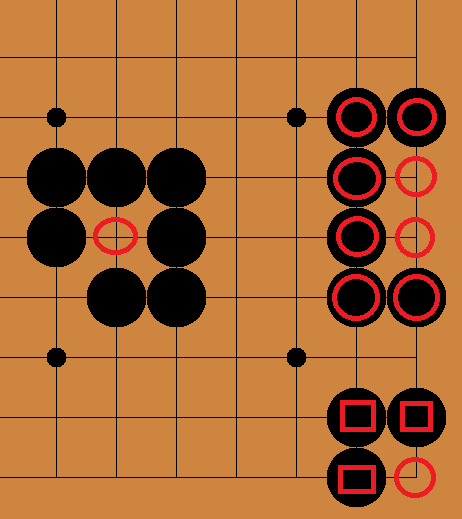
\includegraphics[scale=0.5]{Images/eyes.png}
\caption{Figure 2.1.1 eyes}
\end{figure}

\textbf{Straight Four Eyespace:} A Straight eye of four liberties makes a group alive since white can always make two eyes. The two points labeled 'm' in figure 2.1.2 are miai if white plays one then the black plays the other creating two eyes.

\begin{figure}[H]
\centering
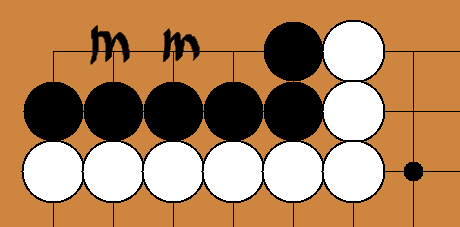
\includegraphics[scale=0.5]{Images/foureyespace.png}
\caption{Figure 2.1.2 striaght four eye space}
\end{figure}

\textbf{Atari:} Atari is a term used in Go for a situation where a stone or group of stones only has one liberty and can be captured on the next move unless the defending player places a stone on the liberty, thus giving the group more liberties and at least temporarily taking the group out of Atari. In figure 2.1.3  if black places a stone at any of the liberties with a red circle then black will capture the white stone. In figure 2.1.4 if white places a stone at either the liberty at “a” or the liberty with a red circle then the black stones will be captured.

\begin{figure}[H]
\centering
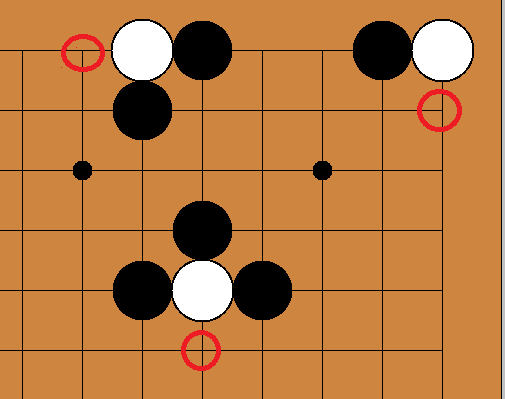
\includegraphics[scale=0.5]{Images/singlestonesinatari.png}
\caption{Figure 2.1.3 single stones in atari}
\end{figure}

\begin{figure}[H]
\centering
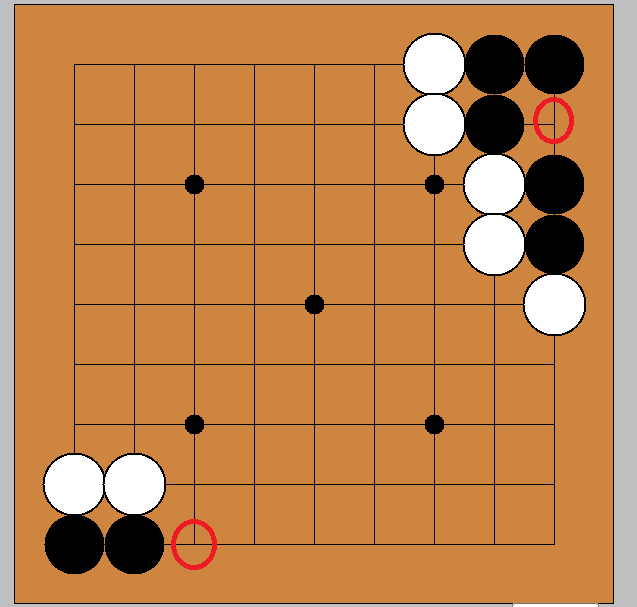
\includegraphics[scale=0.5]{Images/groupsofstonesinatari.png}
\caption{Figure 2.1.4 groups of stones in atari}
\end{figure}

\textbf{Hane:} A hane is either a move that wraps around an opposing player's stone or group of stones and doesn’t touch any of the player’s stones or a diagonal move played in contact with an enemy stone. There are many positions where a hane is considered a good move for example in the six die eight live group of problems which with be detailed later in the chapter. In figure 2.1.5 the stone labelled with a red circle is a hane as it wraps around the black stone and isn’t adjacent to another white stone.

\begin{figure}[H]
\centering
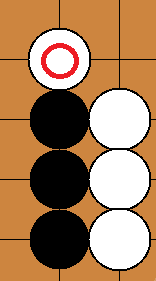
\includegraphics[scale=0.5]{Images/ahane.png}
\caption{Figure 2.1.5 a hane}
\end{figure}

\textbf{Ko:} Ko describes a situation where two alternating single stone captures would repeat the original board position. These alternating captures could repeat indefinitely creating an infinite loop in the game. The Ko rule stops this infinite loop from occurring: If one player captures the Ko, the opponent is prohibited from recapturing the Ko immediately. In figure 2.1.6 above black can capture the white stone with the red circle by a play at “a”. The resulting position is shown in figure 2.1.7. Without a Ko rule, in this position White could recapture the black stone with the red circle by playing at “b”, which would return the board to the position in 2.1.6 and then Black could also recapture creating an infinite loop. So, if in figure 2.1.6 Black captures at “a”, White may not play at “b” for his first move after the black capture. Instead White has to play elsewhere. After that Black can choose either to win the Ko by playing at “b” in figure 2.1.6, or to play elsewhere as well. Playing elsewhere however would allow White to take the Ko back, since the recapture restriction is only valid for the next turn.

\begin{figure}[H]
\centering
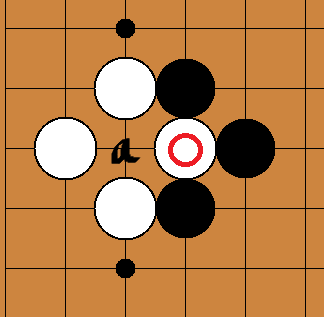
\includegraphics[scale=0.5]{Images/korule2.png}
\caption{Figure 2.1.6 the ko rule part 1}
\end{figure}

\begin{figure}[H]
\centering
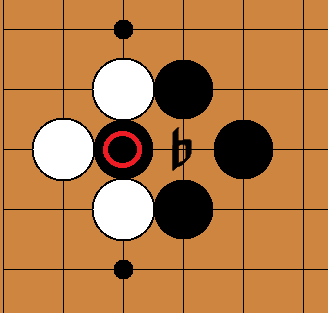
\includegraphics[scale=0.5]{Images/korule1.png}
\caption{Figure 2.1.7 the ko rule part 2}
\end{figure}

\textbf{Miai:} Miai can be defined as a pair of empty points that have the same value. For example if black plays at A, white can play at B and suffer no disadvantage from the exchange. Equivalence is an important aspect of miai, in the sense that the two options allow the same objective to be achieved more or less. For example, miai in a life and death context might mean the existence of two different moves resulting in the same outcome of a group living or being killed. In figure 2.1.8 both point “a” and point “b” have the same value in terms of the life and death of the group if black plays at “a” then white plays at “b” and vice versa. If white places a stone at either “a” or “b” he creates a second eye for the group and thus keeps it alive.

\begin{figure}[H]
\centering
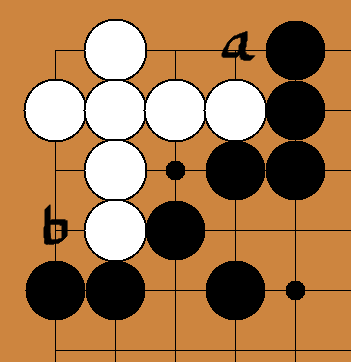
\includegraphics[scale=0.5]{Images/miai.png}
\caption{Figure 2.1.8 miai}
\end{figure}

\textbf{Seki:} The term Seki translated into English means mutual life, this situation occurs when two live groups share liberties which neither of them can fill without dying so neither player will.
 In figure 2.1.9 the white group of stones and black group of stones with red circles share two liberties “a” and “b”. If either player plays into one of these points the opposing player with play into the other and capture the opposing player’s stone so neither player will. [*maybe include another seki example where the group has eyes*] .

\begin{figure}[H]
\centering
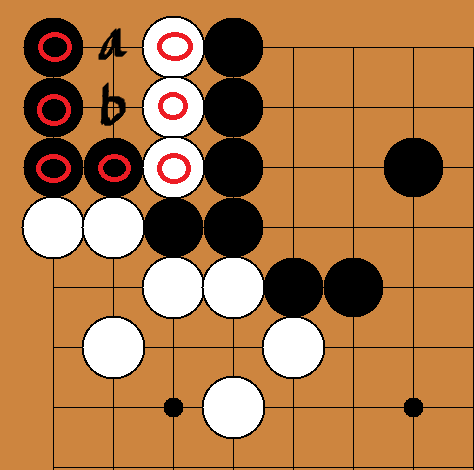
\includegraphics[scale=0.5]{Images/seki.png}
\caption{Figure 2.1.9 seki}
\end{figure}

\section{Go Problems}

\subsection{Why Life And Death?}

As seen by the variety of moves within Go, it is a large and complex game. This extends to the search space for Go's game tree, which is both wider and deeper than that of chess. It has been estimated to be as big as ~$10^{170}$ [reference] compared to ~$10^{50}$ for chess [reference]. It is even possible for the search space for a single life and death problem to be larger than all of chess. As described previously, a life and death problem occurs due to a player's group of stones either being "\textit{alive}" or "\textit{dead}." When a player's group of stones cannot be captured in any game state it is alive, whilst if the opponent is able to capture an opposing group of stones, then that group is dead. Normally, a player will have an objective in mind when playing through a life or death problem - whether it is keeping their group of stones alive or killing an opponent's stones group. With the timescale and number of people working upon this project, creating an AI to play a full sized game of Go would not be feasible. Therefore, the decision to concentrate efforts into solving life and death problems was a more realistic yet still challenging goal. The project initially focused on a small subset of life and death problems before moving on to more computationally challenging problems once the initial problems were being solved with a reasonable success rate.

\subsection{Common Life And Death Problems}

Most life and death problems be grouped into certain shapes or techniques used to solve the problem given the specified objective. These life and death shapes occur frequently during games of Go and in many cases one small positional change of a stone can create a big difference to the outcome of the problem.

\subsection{Unsettled Three}

This shape is concerned with when a group’s interior eye shape consists of three spaces in either the form of a bent three space or a straight three. Here the key number is 3; If the space is any less than three then the group is dead, four spaces and the group is alive. In figure 2.2.1 below, if white plays at either of the red circles the group lives because it creates two eyes for that group. If black plays at either of the red circles it kills white.

\begin{figure}[H]
\centering
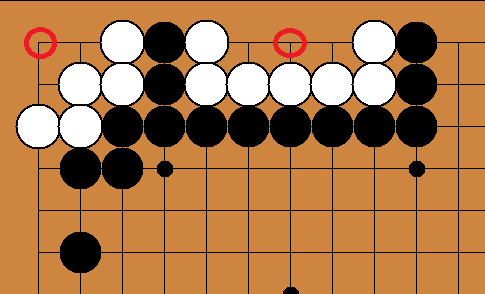
\includegraphics[scale=0.5]{Images/unsettled3.png}
\caption{Figure 2.2.1 eyes}
\end{figure}


\subsection{Six Die, Eight Live}

The groups of stones in this section consist of rows of stones on the second line in from the edge of the board.  Therefore the groups eye space lies on the edge of the board. When the group is away from the corner the rule is six stones die, eight stones live. Figure 2.2.2 above shows the case where the group is alive i.e has eight stones. Figure 2.2.3 shows the case where the group is unsettled i.e has seven stones and finally figure 2.2.4 shows the case where the group has six stones and is dead.

Figure 2.2.3 - Seven is unsettled

Figure 2.2.4 - Six die

\chapter{Design And Implementation}
\label{design}

\section{Requirements Gathering}

At the beginning of the project, a formal specification was given and described the creation of: 
\begin{center}
“\textit{An interactive program, with GUI, that presents a Go problem on a board, and interacts with the user as they explore the solution space of the problem. The program uses tree search algorithms to find good moves}.”  
\end{center}
As this original specification itself was quite brief, several ambiguities were identified in the requirements. These ambiguities included what tasks, goals, and objectives would be explored when designing and implementing the program. Hence, a requirements gathering interview was arranged with the project supervisor, Dr. John O’Donnell, to help specify the requirements further and allow for a thorough plan to be created for the future development of the project. Before the interview, it was already decided that the program would solve life and death problems using the tree search of minimax and alphabeta, due to the reasons specified previously. This meant that the interview questions themselves were targeted at understanding the complexity of solvable life and death problems for the project, the artificial intelligence's capabilities and the production of the graphical user interface utilised by the individual playing through created Go problems. These created questions allowed for a complete problem solver specification as well as an organisation of team member's tasks and milestones at the end of the requirements gathering process to be formed.

\subsection{Interview Questions}

\textbf{Nature Of Problem}

What are the types of objectives the program will be asked to solve?
\begin{itemize}
\item It is hard for the program to determine the nature and goal of a problem as they are laid out in the problem book.  The program would have to choose its own boundary for the problem and determine which pieces are irrelevant to the overall solution of the problem.  This is too ambitious, so a boundary should be defined by the user along with a nominated group of stones that should either be captured or saved.
\end{itemize}
What difficulty of problems (30 Kyu - 9 Dan) should the program be able to solve?
\begin{itemize}
\item It should be able to solve problems correctly at as strong a level as possible.  At a minimum, it should be able to solve simple problems using brute force.  The program should be tested with problems of an estimated strength against a competent human player to find the kyu ranking of the program.  20 - 25 Kyu is around the right ranking that the program should be able to achieve.  If the program ends up better than this, problems of better ranking could be used to improve it further.
\end{itemize}
How complex, as in the number of moves before the solution, should the solvable problems be?
\begin{itemize}
\item The number of moves to solve is a useful metric for calculating complexity when we use a brute force algorithm, however for more complicated heuristics it becomes less useful.  A directory of collections of test cases should be created so that many tests cases are able to be ran over the program and calculate the complexity.  However calibration is difficult as humans and computers find different things difficult.  Humans can perceive “good” moves and can deliberately structure the tree deeper rather than wider by forcing the other player to make specific moves to save their pieces.
\end{itemize}

\textbf{Solution}

How long should the AI have to respond?
\begin{itemize}
\item The program should have no time limit to solve, but it should be reasonable. ie. making a move in a few seconds or minutes compared to days and weeks.  The interface should have a way for the user to define how long the AI has to take a turn as thirty minute turns are too long in practice.  To control time, a difficulty chooser could be implemented that would set time limits for turns or set depth limit for move searches.  This should be a rough guide and not a set limit ie. if the time limit is set to 30 seconds, the AI can take from 10 - 60 seconds. As long as the times are reasonably similar.
\end{itemize}
Whom should the AI be able to play against?
\begin{itemize}
\item It should be able to play against itself or against humans.
\end{itemize}
What minimum success rate should the AI have?
\begin{itemize}
\item The program should be able to solve 28 kyu problems with certainty.  It may be unable to solve 15 kyu problems reliably but may solve them on occasion.
\end{itemize}
How do we know the AI has succeeded?
\begin{itemize}
\item A main group could possibly be elected to either be captured or be saved depending on problem.  If the group is captured, or is unable to be captured then the program could be alerted that the problem has been solved.  Pitting the AI against itself is not a good way to test the successfulness of our program, so the program should be tested with humans who know how to solve the problems so they can pick out problems in the program. There are two avenues that the testing process should pursue, the first being “Small data set; in depth evaluation,” where good “Go” players are asked to make good moves against the AI on a problem and then play again but make bad moves. Then they should be asked if they think the AI is good in the program.  Ideally, there should be 5 (minimum) to 10 (ideal) testers for this step.  The other testing avenue is “Large data set: low depth evaluation,” where a person, aided with the answers to the problems, is asked to test the first move the AI makes of many problems (several hundred). If the AI makes the correct first move, it can be assumed that the program is likely able to find the correct solution.
\end{itemize}

\textbf{Graphical User Interface}

Is a textual user interface required in addition to a graphical user interface?
\begin{itemize}
\item The program could start in TextUI, then have a command to start GUI but the ability to be able to switch between TextUI and GUI is not needed.  A TextUI is important for the portability of the program, as it can be hard to get GUI’s to work on different systems.
\end{itemize}
What information should be shown from the AI?
\begin{itemize}
\item The ability to go back through the moves showing: What moves were considered; What the heuristic evaluated the value of the moves as; Why it did not take moves that would be considered as “good”;  Why it took moves that would be considered as “bad”.  Also, make it possible to query the AI, to ask it what moves it is considering or show the value the heuristic gives for a specific position.  This would help to find the bad decisions in AI so that fixes are more easily targeted.
\end{itemize}

\section{Requirements Specification And Organization}

Following on from the described requirements gathering process involving the conducted interview, a more descriptive requirements specification was created which built upon the originally given project brief: 
\begin{center}
“\textit{The resulting program of this project should be able to solve Life-and-Death Go problems. This should be done either independently by an AI and/or with user interaction via a GUI that shows the board and allows legal moves to be made. The AI should be able to be given an objective such as “defend group A” or “kill group B” for either colour and be able act accordingly. The problem difficulty for the AI to solve should be as high as possible (on a range from 30 Kyu - 9 Dan) and it should solve the problem correctly with a success rate of at least 80\%. This will be assessed by using an unspoiled testing set that meets these requirements}.”
\end{center}

Using this new specification, the planning of the program began. To enable specific design and implementation tasks to be assigned to members, the major components of the problem solver first had to be identified. These components included three separate entities; the game engine, the graphical user interface and the artifical intelligence. I was also decided to split the project into a series of milestones, allowing for the problem solver to be created in accordance with a working deadline. To determine these milestones, several issues were considered. As the GUI and AI could not work without the underlying GameEngine, implementing the GameEngine was to be the first milestone. The AI was identified as being the bulk of the work in this project and hence the GUI was planned to be finished by January during the second milstone. Due to the work needed to implement the artifical intelligence, the basic functionality of the AI was also planned to be completed within this second milestone. Once the GUI and basic AI functionality were implemented, the final section of the program was to implement heuristics for the AI to use to solve many different types of problems.  This was planned as the third and final milestone.

The organisational structure of the team evolved and developed throughout the project. In the first milestone, the GameEngine was split up equally between all members of the team, with each person having a section to implement. This milestone was completed in November when a text based UI was also created so that it was possible to interact with the program before the GUI was implemented. At this point some basic tests were also implemented by everyone in the team on the underlying game engine to ensure that the base of the program was robust. After the game engine was implemented, the team was split into two groups for milestone two. One group, consisting of Eilidh, Jamie, and Scott began working on the GUI whilst the other group, being Kiril and Niklas began working on the basic artifical inteligence functionality.  A working GUI and the MiniMax and AlphaBeta algorithms were completed in January after which some tests were again implemented to guarantee the program was working as intended. For the third and final milestone, the GUI team joined Kiril and Niklas in working on the AI until the end of this project in March.  For this milestone, everyone began work on implementing heuristics for the AlphaBeta algorithm to use to solve different types of problems and evaluating the ability of the program.  During this stage, whilst the GUI was being used some bugs were discovered and some extra functionality was found to be needed.  Therefore part of this milestone was also to iron out these bugs and implement any needed functions.

\begin{figure}[H]
\centering
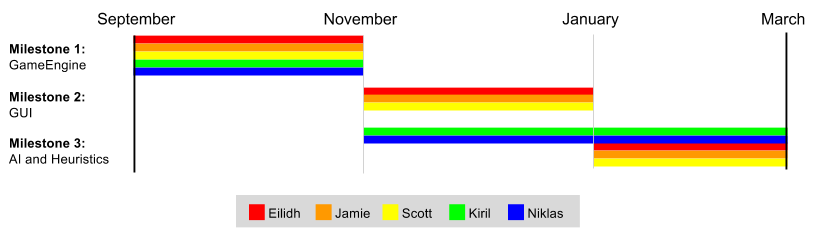
\includegraphics[scale=0.5]{Images/GanntChart.png}
\caption{Gannt chart showing organization timeline.}
\end{figure}

Throughout the project agile software process were used...

\section{Game Engine Design And Implementation}

Upon having established the requirements the first development step was the representation of a board and being able to make exclusively legal moves on it. Further, for the sake of easier interaction, testing and future development, a board loading/saving mechanism and a command-line based UI were also included. This lead to the following basic interaction structure:

\begin{figure}[H]
\centering
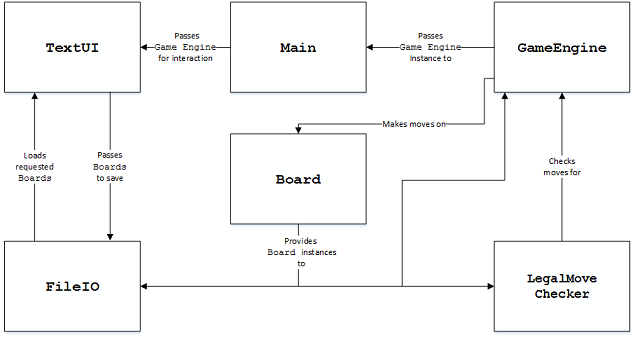
\includegraphics[scale=1]{Images/S33Diagram.png}
\caption{Basic program class structure.}
\end{figure}

Notably, each of these was implemented as a Java class, designed to function as fairly independent components. Their respective details will be discussed henceforth.

\subsection{Main}

This class mainly serves as a runner and was incorporated as it was considered that some initial settings may have to be set prior to launching the UI. It for example, allows one to choose between the TextUI and later developed GUI. Additional settings were considered, but were added elsewhere later on.

\subsection{Board}

The Board class holds the main representation of the board, which is essentially a 2D integer array (type was later adjusted for memory reasons). As each intersection could either be empty or hold a black or white stone, these states could effectively be represented numerically as 0, 1 and 2. Here is an example of this representation:

\begin{figure}[H]
\centering
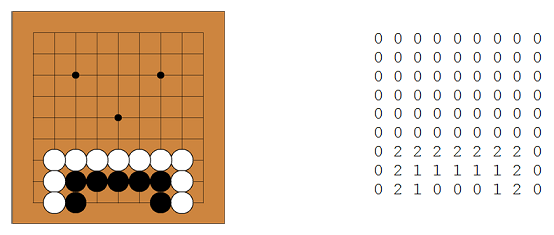
\includegraphics[scale=1]{Images/GE-BoardRep.png}
\caption{Board representation: GUI and TextUI.}
\end{figure}

Notably, a special empty space type (set to 3) was added later on to allow AIs to better determine relevant search areas (See Section 3.5 – Search Scope). The major functions of the board are the setting/getting of intersections, testing for board equality and producing deep copies (clones) upon request. 

\subsection{FileIO}

The FileIO is responsible for reading/writing board states for later usage/testing. Reading in a board state involves verifying its integrity and producing the resulting Board objects, whereas writing converts Boards into writable strings. The file representation of a board does not use integers, but rather characters for the benefit of manual editing (which was necessary prior to the GUI). Accordingly, black, white and empty were represented as ‘b’, ‘w’, ‘.’. Here the previous example:

\begin{figure}[H]
\centering
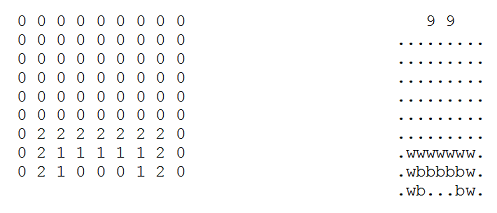
\includegraphics[scale=1]{Images/GE-BoardSave.png}
\caption{Board file representation.}
\end{figure}

The two initial numbers at the start denote the dimensions of the board. This mechanism was further enhanced as the program grew, having files hold further details such as AI search spaces (denoted by ‘-‘) as well as game objectives (E.g “White to kill 2 7”) that instruct the AI as to what group is relevant. Due to the increasing growth, the translation/integrity verification was later moved to a separate translating class.

\subsection{GameEngine}

The GameEngine was designed to be the heart of the program, holding the current Board representation and allowing players to make legal moves on it. In order to check the legality it holds an instance of the LegalMoveChecker that it asks to analyse each move attempted and will only modify the board when said test returns true. Other functions entail undoing moves, restarting the board and other user-oriented features. A further addition that was made later in the project is the addition of AI play and representation. 

\subsection{LegalMoveChecker}

\section{Graphical User Interface Design And Implementation}

To create a fully-fledged Go Problem solver allowing the user to interact with life and death problems, a graphical user interface had to be designed and implemented to allow for communication between the user, GameEngine and artificial intelligence. The finished GUI was created using Java Swing [reference here] and the Graphics package [reference here]. The user interface provides a wide range of functionalities through graphical board representation and the implementation of interactions such as placing stones and saving board states. Hence the final design of the GUI successfully allows the user to create and play life and death problems as specified within the requirements.

\subsection{Initial Design}

During the preliminary design process of the GUI, a paper prototype was created as a basis for implementation. As can be seen in Figure 3.1, the paper prototype showed the original layout of the user view of the GUI which consisted of several elements. These elements included a representation of the board, featuring white and black stones where the human and AI would both play moves. Another component that can be seen are the radio buttons that were drawn out, which would allow the human and computer's stone colours to be chosen. Lastly, an undo button and a reset button were also included in the paper prototype. The undo button would remove the latest move on the board, whilst the reset button would adjust the board back to its original loaded state. The original design also included a toolbar featuring a single button, labelled "Menu".  Pressing the menu button reveals the options seen in Figure 3.2 for loading and saving the board, as well as saving a log which would be a series of played moves. Whilst the paper prototype was a strong basis for the beginning of implementation, it was missing a wide range of functionalities, such as bounds and player modes which were included within the final implementation. Some redundant options within the original paper prototype's file menu were also removed during implementation, such as the save log.

\begin{figure}[H]
\centering
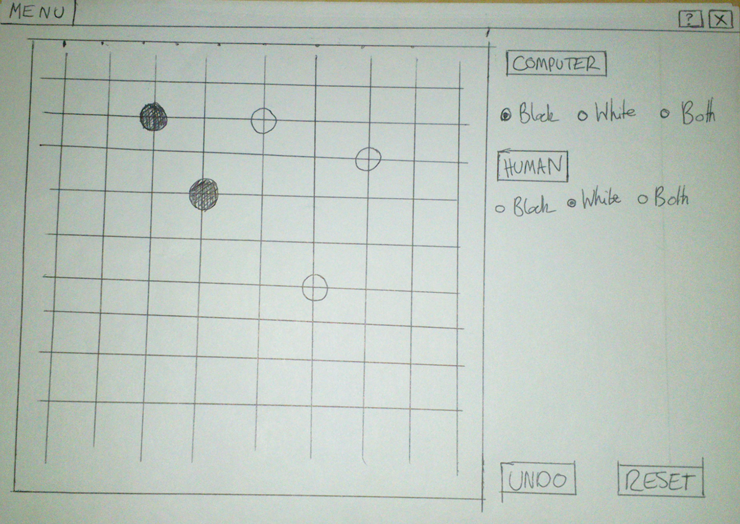
\includegraphics[scale=0.4]{Images/GUI-1-PP.png}
\caption{Original paper prototype GUI view.}
\end{figure}

\begin{figure}[H]
\centering
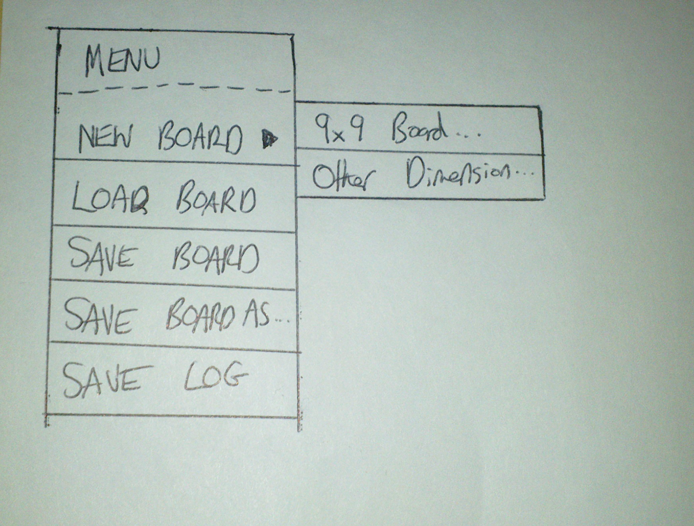
\includegraphics[scale=0.4]{Images/GUI-2-PP.png}
\caption{Original paper prototype file menu.}
\end{figure}

\subsection{Visual Implementation}

The first step of implementing the GUI was the graphical board representation, which can be seen as the main visual feature of the problem solver. As described previously (see \textit{Section 3.3}), the GameEngine uses a 2D array to represent the board within a Board object. This 2D board array had to be translated to a graphical representation to enable the GUI to communicate directly with the GameEngine and AI as well as the user. As the GUI was created using Java Swing [reference here], the Graphics package [reference here] was utilized to provide a visual of the board. To depict the board on screen, the current number of board lines (height/width) are taken from the Board object specified within the GameEngine. A series of brown rectangles are then drawn and filled in to represent the board using the number of specified board lines. These rectangles overlap to form the appearance of a grid and again using the line number provided, coordinates are drawn aligned to each of the rectangles. The user can control whether these coordinates are shown or not and they can be a useful aid during play. This described method of drawing out the board means that the GUI is flexible to representing any size of board specified by the user, as long as it is a square. Following on from the successful drawing of the board layout itself, the GameEngine's 2D array board representation is scanned and when a stone was found - being Integer 1 for black and Integer 2 for white - the appropriate counter is drawn on the board. The counters are painted in a top-left across and down fashion, comprising of a fully coloured circle with a given edge around them. Hence, a full board containing a grid, counters and available coordinates is drawn as seen in Figure 3 using the 2D Board object array provided to the GUI.

\begin{figure}[H]
\centering
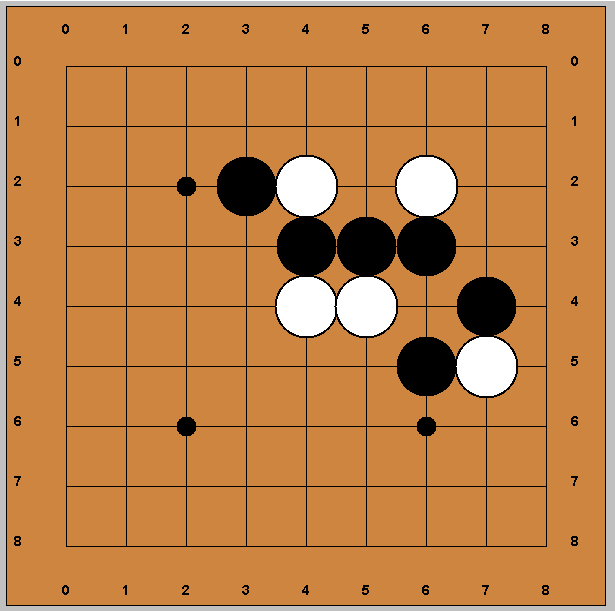
\includegraphics[scale=0.5]{Images/GUI-3-CountersCoords.png}
\caption{Full board (grid, counters and coordinates).}
\end{figure}

Several other visual enhancements were made following the original drawing of the board, allowing for a higher level of feedback and a more user-friendly system. These included the use of transparent stones upon the board when the user's mouse hovers over an intersection showing where a stone can be placed upon the board. These transparent stones are colour-coded and are either black, white or red - which signifies an illegal move through the utilisation of the legal move checker, an important part of the GameEngine as described previously (see Section 3.3). The see-through stones are depicted in Figure 4 and were also implemented using a 2D array, likewise to the current board representation. This 2D array refreshes itself each time a mouse move is detected. After this refresh, a stone is placed within the transparent stone's 2D array at the current location of the mouse. Checking whether the current stone location is legal or not occurs after the updating of the 2D array and once the check occurs, the appropriately coloured see-through stone is displayed.

\begin{figure}[H]
\centering
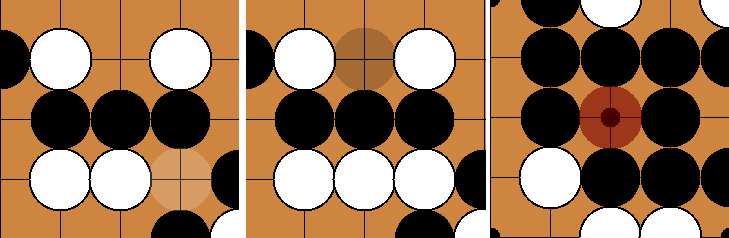
\includegraphics[scale=0.7]{Images/GUI-4-Transparent.png}
\caption{Transparent stone: White, black, illegal move.}
\end{figure}

Yet another visual enhancement within the GUI can be seen in Figure 5, being the depiction of the artificial intelligence's search space as bounds. These bounds are depicted graphically and represent the board positions that the AI will consider moving to. The intersections that are available to the AI are coloured brown, whilst the rest of the board is greyed out. This graphical feedback allows the user to easily see the multiple positions which the computer will possibly move to and this feedback can be toggled on or off according to the user's preference. Originally the bounds took only the shape of a rectangle or square between two specified user points, however through a process of improvement the finished GUI allows the user to select a flexible set of bounds simply by clicking on the intersections to be included within the AI's search space. This change not only provided better visual feedback but was also more efficient for running the artificial intelligence whilst in-game.

\begin{figure}[H]
\centering
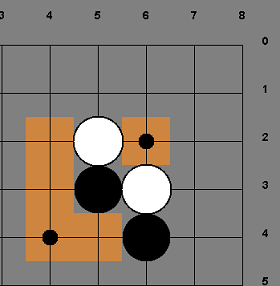
\includegraphics[scale=1]{Images/GUI-5-Bounds.png}
\caption{Artificial intelligence's graphically represented bounds.}
\end{figure}

\subsection{Player Modes}

Following the implementation of the board representation itself, as well as several other visual features, a major design change from the paper prototype took place. The design decision was made to implement two separate user playing modes, being "\textit{Creation Mode}" and "\textit{Competitive Mode}." The availability of user modes allows for easy distinguishing between the two main features of the Go problem solver - being allowing a player to create a problem or playing out a problem. The creation of a problem provides the user with various options whilst playing out a problem allows the user to choose between playing against the AI or another human. The separation of the two modes also rids the GUI of the possibility of having overlap of certain features between modes, which could create numerous errors. For example, deletion of stones is only available in creation mode. Each mode also has their own dedicated menu upon the toolbar, named "\textit{Problem Creation}" and "\textit{Competitive Play}."
When the GUI is initially started, it is opened in problem creation mode and displays a blank 9x9 Go board ready to begin letting the user design their own life and death problems. The problem creation menu in the toolbar, as seen in Figure 6, allows access to various features during the creation of problems within the GUI. These include options for the placement of stones, such as using only a specific colour of stone (white/black) or being able to delete stones by pressing on them. Problem creation mode also allows the user to alter the AI's objective and bounds. The objective is specified in a pop up box, as displayed in Figure 7, whilst the bounds can be altered by the user selecting bound selection and then specifying their bounds by selecting specific intersections. This collection of features easily allows for problems to be made quickly and can then be saved by the "\textit{Save Problem}" option in the file menu, ready to be played in competitive mode.

\begin{figure}[H]
\begin{subfigure}[H]{0.2\textwidth}
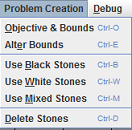
\includegraphics[scale=1]{Images/GUI-6-PCMenu.png}
\caption{Problem creation menu.}
\end{subfigure}
~~~~~~~~~~~~~~~~~~~~~~~~~~~
\begin{subfigure}[H]{0.3\textwidth}
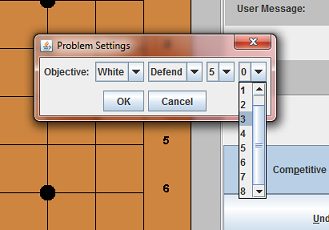
\includegraphics[scale=1]{Images/GUI-7-Objective.png}
\caption{Objective dialog choice box.}
\end{subfigure}
\caption{Creation mode user options.}
\end{figure}

Competitive mode meanwhile is intentionally selected by the user after the initial opening of the GUI. This mode allows for the play through of a problem in several approaches, including human versus human, human versus AI (either Minimax or AlphaBeta) and AI versus AI. Upon selection of the "\textit{Competitive Mode}" button a pop up box appears allowing for player choice as seen in Figure 8. If the bounds and objective are not specified before this selection, the GUI will prompt the user to choose them before allowing competitive mode to be entered. Once a game is in play, the problem creation menu is greyed out and the competitive play menu is available to use. This menu includes such features as swapping player colours, forcing the AI to move and also allowing the user to change the AI type currently being used within play. An example of an AI move can be seen in Figure 9 and Figure 10, where labels on the side of the board specify the AI type and its move selection which allow the user to easily learn from its position selection, as seen in Figure 11. *WRITE ABOUT HEURISTIC CHOOSER HERE* Hence the options available in competitive mode allow for a flexible and user friendly environment whilst playing through a problem with the user interface.

\begin{figure}[H]
\centering
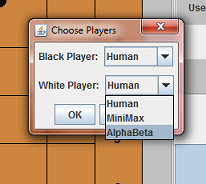
\includegraphics[scale=1]{Images/GUI-8-PlayerChoice.png}
\caption{Player dialog choice box.}
\end{figure}

\begin{figure}[H]
\centering
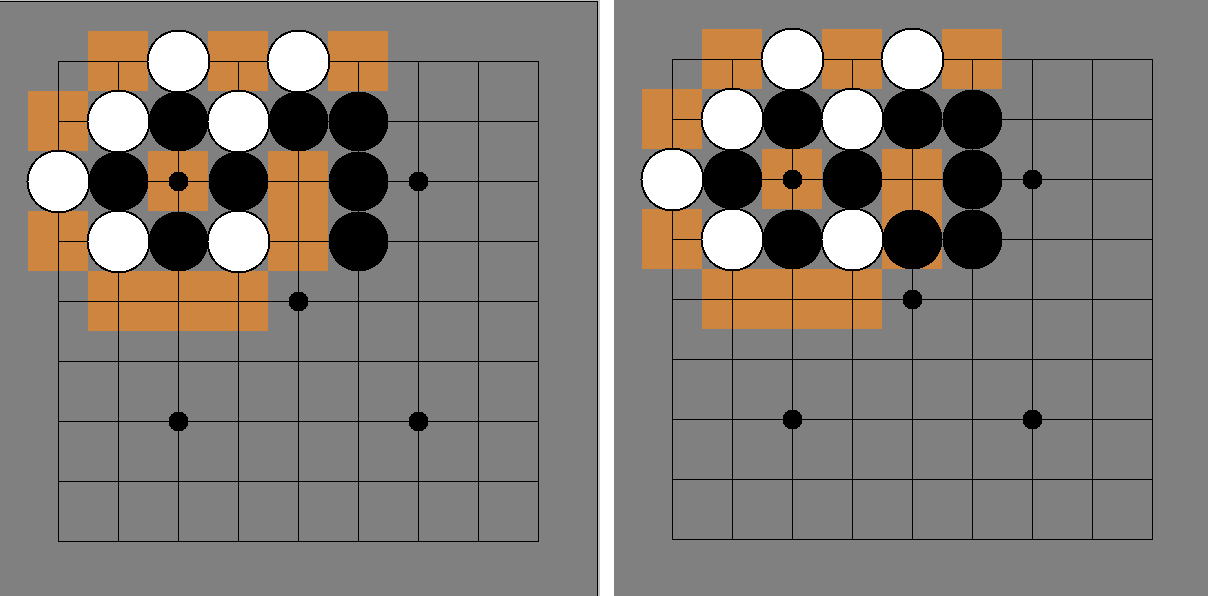
\includegraphics[scale=0.5]{Images/GUI-9-AIMove1.png}
\caption{Example of AI moving (successfully capturing black stones).}
\end{figure}

\begin{figure}[H]
\centering
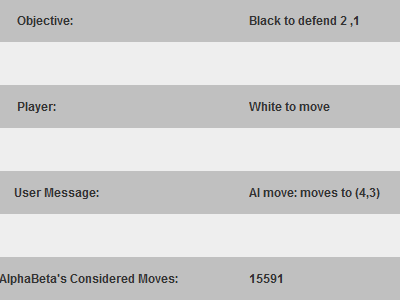
\includegraphics[scale=1]{Images/GUI-11-AIMove3Feedback.png}
\caption{AI feedback following its move.}
\end{figure}

\textit{Insert heuristic chooser picture}

Several features of the GUI are included in both creation and competitive modes. These features include the "\textit{Show Coordinates}" button which displays the coordinate numbers along all sides of the board, allowing easy stone placement. The user can also load or save problems at any point as well as using debug features. Debug features include displaying the log, being the history of all actions within the GUI. Also, the usage of the help menu is available in both modes which has options including the display of keyboard shortcuts. For example making the AI move against itself in AI versus AI mode can be quickly done using \textit{ALT + I} and there are several other keyboard shortcuts which enable even quicker use of the GUI. Other useful functionalities provided in both modes include the undo and reset button, allowing for the quick backing up of mistakes or reset to the original board, which is practical at all times for the user.

\subsection{Finalised Graphical User Interface}

Through the evidence given prior, it is clear that a user interface was completed successfully allowing for easy interaction during problem creation and competitive play. The entire finished view of the GUI can be seen in Figure 12. The final implementation of the interface allows for the quick creation and saving of problems before the user is able to play them in a variety of ways and against several different entities, including the AI and other human players. The GUI also has a wide range of useful features, such as making the AI's functions, including search space and heuristics, available to the user, as well as having a clean look and layout.

\begin{figure}[H]
\centering
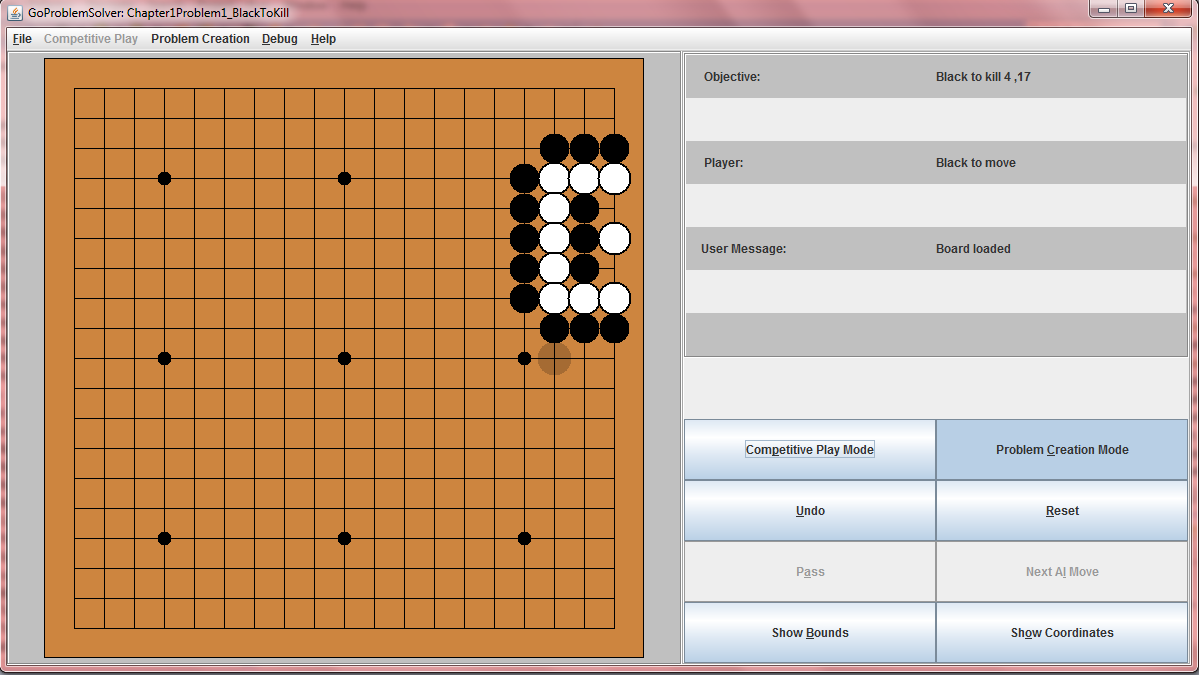
\includegraphics[scale=0.5]{Images/GUI-13-FullView.png}
\caption{Full view of the final GUI.}
\end{figure}

\section{Artificial Intelligence Design And Implementation}

The aim of our program is to play interactively with the user through a solution of a given life and death problem. In order to do that, the program needs to be capable of solving the problem by itself. Accomplishing this required an artificial intelligence, which can make humanlike moves, to be created.
 
Typical life and death problem involves a board position and an objective to be achieved. The aim of the artificial intelligence is to find a sequence of moves in the given situation that satisfy this objective. This gives the program the ability to respond properly to any move made by the user (or by the program itself in AI vs AI game mode). Therefore, developing such artificial intelligence was of major importance. There are several ways it could be implemented by and one of them relies on using a tree search algorithm like Minimax or Alpha-Beta.
 
A tree search algorithm considers each possible action at a given moment alongside each of the subsequent possible actions and so on until a state is found that satisfy a given goal. This allows for brute-forcing of life and death problems in an attempt to find a winning sequence of moves. When the search reaches a state where the objective is completed or where there is no chance to complete it anymore, the corresponding result is returned and the move with highest score is picked. Since all possible moves are considered, the larger the number of possible moves, the slower the response time of the AI. Therefore, to get a decent result in reasonable time, the program should not deal with problems that involve considering a large number of legal moves.

\subsection{Minimax: Design And Implementation}

In games like Go where two players are involved the search tree algorithms become more complicated. They have to take into account the assumption that the opponent also chooses the move that gets the best result. That is the case with the Minimax search, where there are two types of nodes – a max and a min node. The max node is where the player tries to maximize his score and the min one is where the opponent attempts to minimize his. The leaf nodes are the terminal positions of each sequence and contain a value illustrating the result of the particular sequence. Starting from there and going up the tree the max nodes get the maximum value of its children and the min nodes get the minimum of its children nodes. At the end, the root stores the value of the best move at that moment.  

Our implementation of the Minimax follows the stated description, but the actual tree is not constructed. Instead, each move is created recursively. The type of the AI (either Minimax or Alpha-Beta) is chosen from the GUI by the user. If the Minimax is selected it is instantiated and gets a stone colour as well as the objective for the current problem.  
On every move that the computer has to make it gets the current board and runs a recursive function for every legal move it finds with the help of the Legal move checker. The next step of the recursion is to consider every legal response that the opponent could perform and so on until a terminal state is found where either the computer wins, loses or just can not improve the situation by placing stones and has to pass. The values of the outcomes are then passed back and the results of all the initial moves are compared. The move with the highest result is chosen as a reply and its board coordinates are given to the game engine to actually perform the move.

A significant improvement was made during the implementation of the algorithm. Initially in the design on every recursive move generated a separate function had to create all the possible boards, which was found inefficient. It was replaced by a loop which iterates over the board and when a legal move is found the recursive function is called for that move.


\subsection{AlphaBeta: Design And Implementation}

Alpha-Beta search is almost similar to the Minimax. In fact they are guaranteed to always give the same result, but Alpha-Beta has better performance, since some of the branches are not investigated. The algorithm maintains two values, alpha and beta, which represent the maximum score that the maximizing player is assured of and the minimum score that the minimizing player is assured of respectively. Initially both players start with their worst possible score - alpha is negative infinity and beta is positive infinity. It can happen that when choosing a certain branch of a certain node the minimum score that the minimizing player is assured of becomes less than the maximum score that the maximizing player is assured of (beta<=alpha). In that case, the parent node should not choose this node, because it will make the score for the parent node worse. Therefore, the other branches of the node do not have to be explored. This property of the algorithm decreases significantly the time needed to find a good move when brute-forcing life and death problems.

Our implementation of the Alphabeta does not differ much to the one of the Minimax. Again the actual tree is not constructed. The values of alpha and beta are maintained in order to break a particular recursion if the situation described in the previous paragraph occurs – beta becomes less or equal to alpha. The connection of the Alpha-Beta with the other components in the program is the same as for the Minimax.

\section{Heuristics Design And Implementation}

Move selection through minimax and alpha-beta allows for a variety of problems to be solved when making use of brute force alone. However, the more complicated life and death problems take a huge amount of time due to the number of exhaustive moves considered and there is no real strategy used by the program when choosing moves in the brute force case. Hence, to improve the performance of the problem solver, a wide range of heuristics were also implemented to be used in conjuction with alpha-beta. Heuristics were used to provide the artifical intelligence with game strategies and are fundamental to the creation of a problem solver which is more able to mimic a human player's thought process during play. They allow the AI to quickly pick out moves through the implementing of evaluation functions which recognize specific patterns and highlight strong moves algorithmically. In effect, this enables the artificial intelligence to play more effectively against a human with previous knowledge of life and death problems tactics.

\subsection{General Heuristics}

\subsection{Specific Problem Heuristics}

\section{Integration And Implementation Reflection}

As described previously, the finished Go problem solver is made up of a series of components - namely the GameEngine, GUI, AI and heuristics. Each of these components had to be integrated together and given communication abilities to create the finalised program. Once integration had occurred, a simple reflection was carried out, allowing insight into any design or implementation changes that would have been made given more preparation time.

Before the implementation of heuristics; the GUI, AI and GameEngine were created separately and then integrated together. The GameEngine easily interacts with the AI through the use of a private AI variable, allowing the GameEngine to access AI search space, the AI type and AI move selection. The more difficult integration was matching the GUI against the GameEngine and hence allowing it to communicate with the artificial intelligence. Despite the difficulties, this was achieved effectively before heuristics were implemented. The integration was carried out by matching GameEngine methods to GUI buttons and several methods were also added to the GameEngine to allow the GUI to directly interact with the AI instance. After integration, a range of bug fixing occurred and the visual representation of the artificial intelligence within the GUI made it easier to identify problems. Heuristics were then added to the AI later and integration was relatively simple in this respect. Figure 1 shows the interaction between the finalised components and the success of integration can be seen clearly.

*TBA: ADD FIGURE 1 (UML Diagram of finished implementation/integration)*

Looking back upon design, implementation and integration there are several design choices and processes that may have been different with more time availabilty. For example, if this were a long-running Go project several more heuristics would have been design and coded to allow for a more strategic artificial intelligence. Such heuristics include *ADD HEURISTICS/EXPLANATION* Also, in terms of board representation the choice of a 2D array was probably not the wisest design choice and a data structure such as a hash map may have allowed for a faster running program and less confusion about the laying out of coordinates within the array. Other design choices that can be reflected upon also include more features within the GUI, such as a more realistic board which could have been created using web-coding, for example HTML \cite{HTMLRef}, or a different Java package that was not Java 2D [reference here]. Another GUI feature that could have been added include allowing the AI to run against itself automatically without being prompted against the user. *ADD AI EVALUATION HERE* Hence, there were several design and implementation choices identified after integration that could have been benefitted from a different approach and these were expanded on during the evaluation process (see \textit{Section 5}).

\chapter{Evaluation}
\label{evaluation}

\section{Solvable Problems}

To determine the level of quality of the final Go problem solver created, a series of evaluation techniques were carried out. As the original requirements required a problem solver that can solve life and death problems, the most deterministic approach of measuring the success of implementation was through finding life and death problems that the finalized program could successfully complete. Also found were several unsolvable problems that the program could be extended to solve in future through added heuristics. Both types of problems identified during evaluation have been included in "\textit{Solvable Problems}" and "\textit{Unsolvable Problems}" directories that come with the problem solver. These directories are automatically displayed when the "\textit{Load Problem}" option is chosen under the file menu, hence allowing user access to the problems found during evaluation.

\subsection{Solvable Problems With Brute Force}

Using brute force alone, several life and death problems were able to be solved by the problem solver.

Add examples of solvable brute force problems (Include difficulty estimates/time to solve)

\subsection{Solvable Problems With Heuristics}

Once brute force was extended through the use of heuristics, as described in \textit{Section 3.6}, the program was able to solve several new, more specialised problems.

Add examples of solvable heuristic problems (Include difficulty estimates/time to solve)

\subsection{Not Yet Solvable Problems}

Aside from solvable problems, there are also an array of unsolvable problems that the problem solver could be extended to be able to solve in future. \textit{Section 3.7} describes several heuristics that could be added with further development, and the following unsolvable problems relate to these specific heuristics.

Add examples of not yet solvable problems (Include difficulty estimates)

The original requirements (detailed in \textit{Section 3.2}) desired a problem solver which could solve 15 Kyu problems, being of around a median difficulty, and a success rate of 80% in dealing with this problems. The collection of solvable problems found of varying difficulty prove the success of these requirements. Whilst it is hard to determine the percentage of the program's success rate, as the number of life and death problems is virtually endless, the large collection of solvable problems found does prove that the combination of artificial intelligence and heuristics has enabled the creation of a capable problem solver which will allow human players to work upon their strategy and play through life and death problems outwith a full game of Go.

\section{Subject Testing}

Whilst evaluation through the finding of solvable problems was carried out by the team itself, testing using subjects outwith the team was also performed and provided valuable feedback. A testing document was prepared (see Appendix [insert number here]) and was given to participating test subjects. The document asked the tester to input a set problem given, or their own problem, into the program and attempt to run it in a mode of their choice: AI vs. human, AI vs. AI or human vs. human. Following this, the testers were asked to write down their feedback on the general problem solver, as well at its two modes: problem creation and competitive play. Before beginning testing, participant's consent was acquired, they were given the team's contact details and they were also informed them they could withdraw at any point during testing. Once testing was complete, the testers participated in a discussion focused on the evaluation. Hence, subject testing was carried out as required by ethics procedures.

\subsection{General Interface Testing}

Through the evaluation conducted by real life subjects, a wide range of feedback was supplied concerning the general interface of the problem solver itself, including graphical representation and layout.

Insert interface feedback/evaluation

\subsection{Problem Creation Mode Testing}

As described above, participants were asked to create a problem within the problem solver during problem creation mode. The problem itself was simple and required a range of white and black stones, as well as user set objective and bounds. User attempts at problem creation provided a wide range of feedback relating to the creation of problems within the problem solver.

Insert problem creation mode feedback/evaluation

\subsection{Competitive Play Mode Testing}

The testing subjects were also asked to play through the problem they had previously created using competitive play mode. They were asked to use any specific mode they wished (human vs. human, AI vs. human, etc.) and provide written feedback on their selection and thoughts on play through following their use of competitive mode.

Insert competitive mode feedback/evaluation

\section{Other Testing}

The most valuable evaluation feedback for the Go problem solver was provided through the finding of solvable problems and user testing, as described above, but other miscellaneous testing also helped to prove the program's degree of success as well as improve it during actual implementation.

Insert description of JUnit tests/attempted bug finding, etc.

\section{Testing Overview}

Overall, a wide variation of testing procedures were carried out using the program, both during development and following its completed implementation.

Describe outcome of solvable problems (number of found problems)/highlight recurring user feedback/reiteration of other testing

\chapter{Conclusion}
\label{conclusion}

*ADDING CITES HERE JUST NOW SO BIBILOGRAPHY DISPLAYS*
\cite{2DAPI,Swing,Graphics,BeginnerGo,GoProbs,AI,MCG}

\bibliographystyle{plain}
\bibliography{TeamIDissertation}

\chapter{Appendix}
\label{appendix}

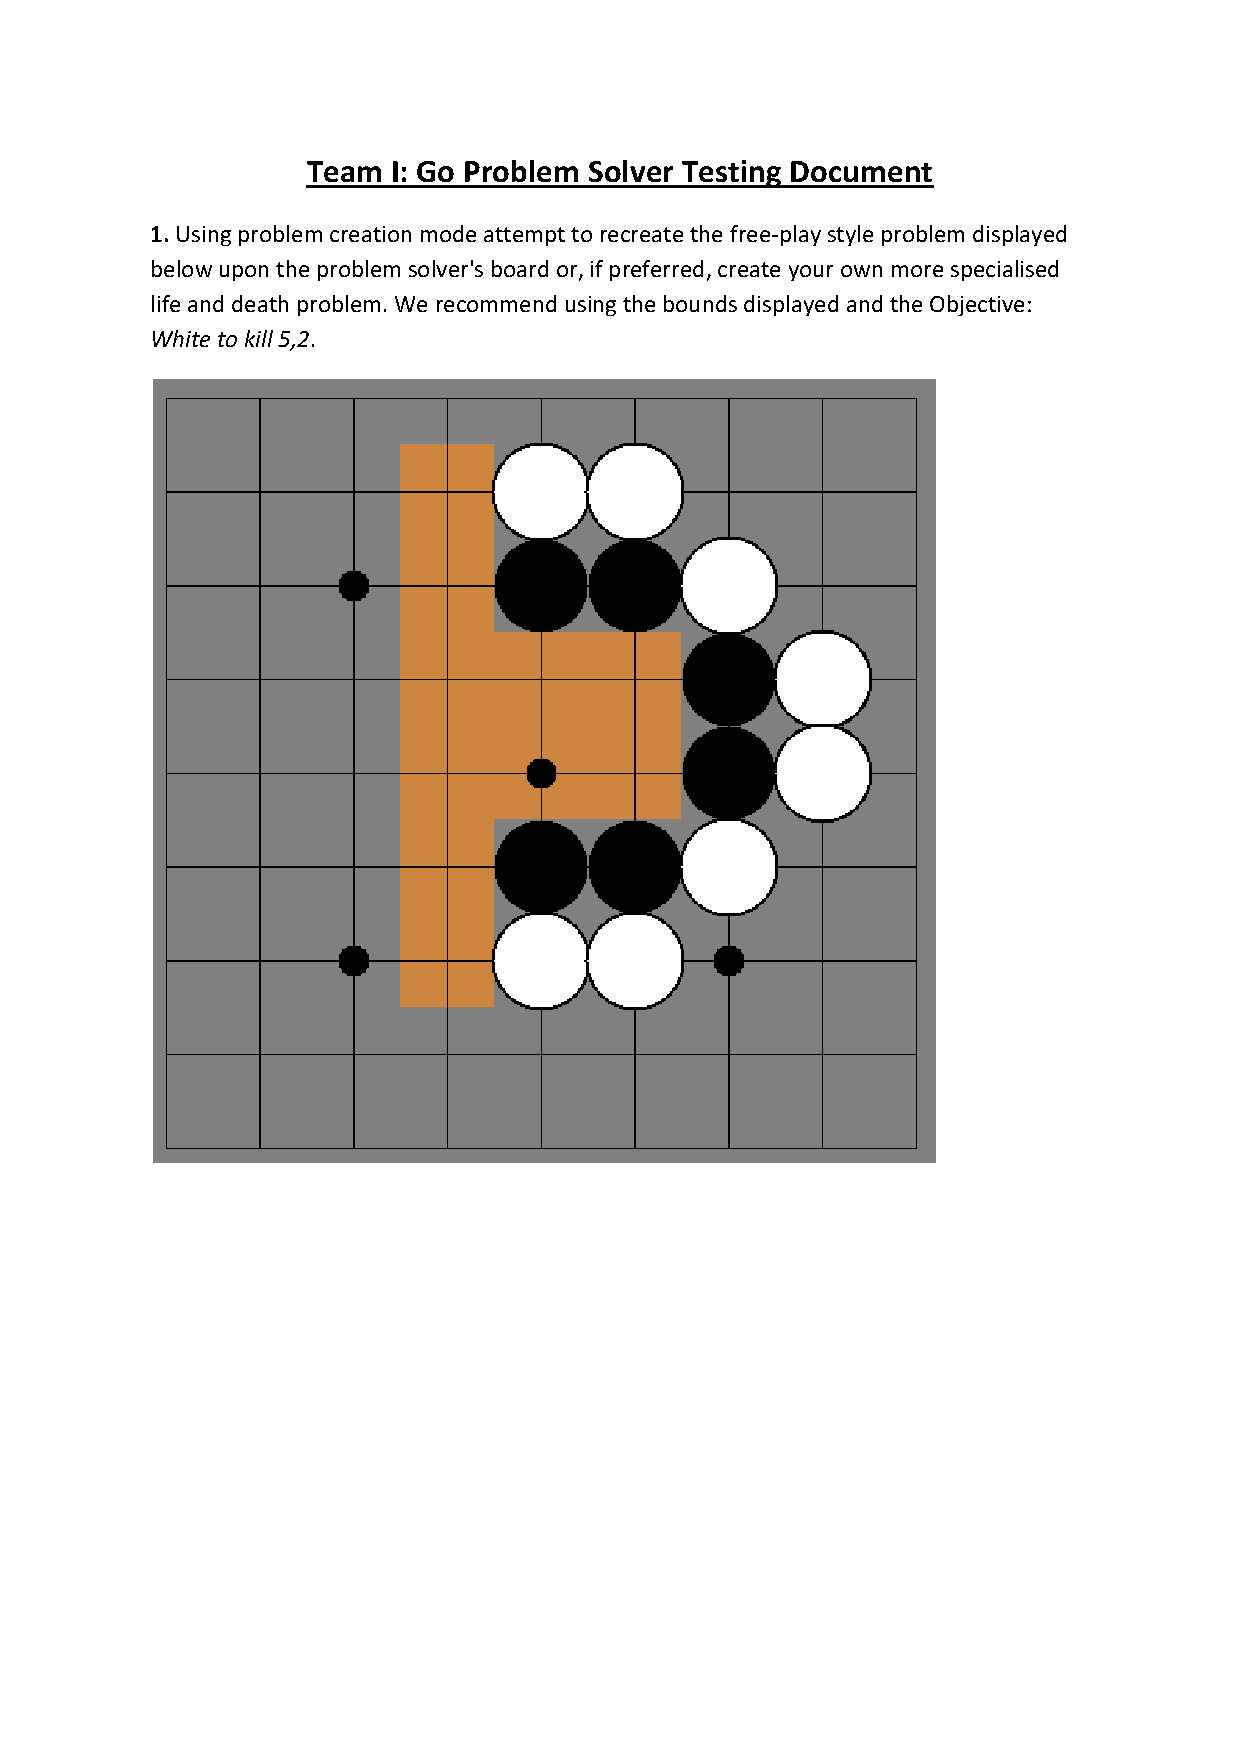
\includepdf[pages={1,2,3,4}]{Appendix/TestingDocumentPDF.pdf}

\end{document}
